\documentclass{beamer}
\usepackage[utf8]{inputenc}

\usetheme{Madrid}
\usecolortheme{default}
\newcommand\tab[1][1cm]{\hspace*{#1}}

%------------------------------------------------------------
%This block of code defines the information to appear in the
%Title page
\title[Verificare formala] %optional
{Proiect}

\subtitle{Verificare formala}

\author[] % (optional)
{Pinghireac Bogdan, Eduard Marian Neguriță, Andreea Bîra-Negrut, Larisa Drăgănescu, Elber Xavier}
\institute[UVT] % (optional)
{
  \inst{1}%
  UNIVERSITATEA DE VEST DIN TIMI\c SOARA
  \and
  \inst{2}%
  FACULTATEA DE MATEMATIC\u A \c SI INFORMATIC\u A
}

\date[2023] % (optional)
{2023}

%End of title page configuration block
%------------------------------------------------------------



%------------------------------------------------------------
%The next block of commands puts the table of contents at the 
%beginning of each section and highlights the current section:
%------------------------------------------------------------


\begin{document}

%The next statement creates the title page.
\frame{\titlepage}


%---------------------------------------------------------
%This block of code is for the table of contents after
%the title page
\begin{frame}
\frametitle{Cuprins}
\tableofcontents
\end{frame}
%---------------------------------------------------------


\section{Introducere}

%---------------------------------------------------------
%Changing visivility of the text
\begin{frame}
\frametitle{Introducere}
\tab In aceasta lucrare este vorba despre rularea unui benchmark folosit 2 tool-uri si anume: Marabou si $\alpha$,$\beta$-Crown folosind setul de date traffic-sign-recognition. \\
\tab Vom prezenta pe rand cum se instaleaza tool-urile si in ce mediu de lucru functioneaza si de asemenea ce programe/librarii sunt necesare pentru o rulare optima si corecta. \\

\end{frame}

%---------------------------------------------------------

%---------------------------------------------------------

\section{Dataset}

%---------------------------------------------------------
%Highlighting text
\begin{frame}
\frametitle{Dataset}
\tab Am optat pentru setul de date Traffic Sign Recognition Benchmark datorită recunoașterii sale remarcabile în domeniul semnelor de circulație. \\
\tab Configurația setului de date evidențiază importanța unei clasificări precise a semnelor de circulație. Fiecare categorie de semn, inclusiv "Limita de Viteză", "Oprire" și "Cedează Trecerea", este asignată unui dosar dedicat. \\
\tab Folosind aceasta structura se optimizeaza procesul de cautare al datelor, fiind un factor esential in ceea ce priveste invatarea eficienta a modelelor de recunoastere. In acest se de date se gasesc semne de circulatie cu forme, culori si dimensiuni diferite acoperind scenarii din mediul urban cat si rural.
\end{frame}

%---------------------------------------------------------

\section{Instalare Tool-uri}
%---------------------------------------------------------
%Two columns
\begin{frame}
\frametitle{Instalare Tool-uri - Alpha Beta Crown - Introducere}

\subsection{Alpha Beta Crown}
\subsubsection{Introducere}
\tab Alpha Beta Crown sau $\alpha$,$\beta$-Crown este un tool care verifica o retea neuronala construit pe un cadru care utilizeaza propagarea liniara legata si tehnici de ramificare legate. \\
\tab Tool-ul este foarte eficient daca este folosit cu un GPU deoarece are mai multe resurse decat un CPU si astfel executia este mult mai rapida. De asemenea se poate scala in mod eficient la retele convoluționale de dimensiuni semnificative, inclusiv cele cu milioane de parametri. \\
\tab Este compatibil cu o varietate extinsă de arhitecturi de rețele neuronale datorita bibliotecii auto\_LiRPA dezvoltate de acceasi echipa. \\
\tab Algoritmul LiRPA foloseste de asemenea un algoritm grafuri computationale generale definite prin intermediu PyTorch.

\end{frame}
%---------------------------------------------------------
\begin{frame}
\frametitle{Alpha Beta Crown - Instalare}

\subsubsection{Instalare}
\tab Pentru instalare avem nevoie de un sistem de operare Linux(noi am utilizat Ubuntu 22.04) si urmatoarele programe/librarii instalate, altfel se pot genera erori:
\begin{itemize}
  \item git
  \item unzip
  \item nvidia driver
  \item cuda tool-kit
  \item anaconda sau miniconda
\end{itemize}
\tab Urmatorul pas este clonarea repository $\alpha$,$\beta$-Crown(\href{https://github.com/Verified-Intelligence/alpha-beta-CROWN}{link}), auto\_LiRPA(\href{https://github.com/Verified-Intelligence/auto_LiRPA}{link}) si vnncomp2023\_benchmarks(\href{https://github.com/ChristopherBrix/vnncomp2023_benchmarks}{link}). $\alpha$,$\beta$-Crown si vnncomp2023\_benchmarks trebuie sa fie in acceasi locatie iar auto\_LiRPA se va clona in folderul alpha-beta-crown.
\end{frame}
\begin{frame}
\frametitle{Alpha Beta Crown - Instalare}

\tab Dupa clonare trebuie realizat enviroment-ul general. In repository-ul de alpha-beta-crown exista un tutorial pentru creare enviroment si un script de rulat si anume:
\begin{itemize}
  \item "conda env create -f complete\_verifier/environment.yaml --name alpha-beta-crown" - care de asemenea va instala din librariile necesare pentru rulare.
  \item "conda activate alpha-beta-crown" - pentru activarea enviroment-ului specific unde se vor instala alte librarii
  \\
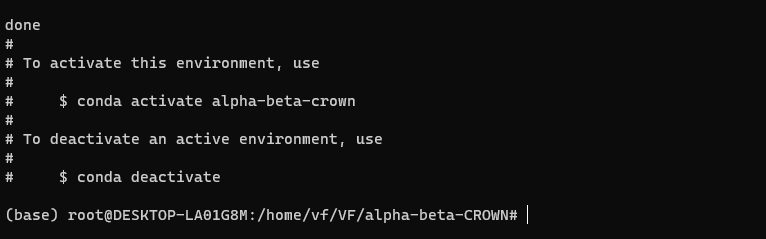
\includegraphics[width=8cm]{2.png}
\end{itemize}
\end{frame}
\begin{frame}
\frametitle{Alpha Beta Crown - Instalare}

\tab Dupa acest pas intram in folderul auto\_LiRPA si rulam scriptul setup.py cu urmatoarea comanda:
"python setup.py install"\\
\tab Apoi mergem in folderul vnncomp2023\_benchmarks unde trebuie rulat setup.sh (atentie sa aveti instalat unzip altfel vor aparea multe erori!!). Rularea poate dura destul de mult timp(depinde de viteza de internet) deoarece se vor descarca multe fisiere.\\
\end{frame}
\begin{frame}

\subsection{Marabou}
\frametitle{Marabou - Introducere}

\subsubsection{Introducere}
to be done
\end{frame}
\begin{frame}

\frametitle{Marabou - Instalare}

\subsubsection{Instalare}
to be done
\end{frame}

\begin{frame}

\frametitle{Rulare benchmark - Alpha Beta Crown}

\section{Rulare benchmark}
\subsection{Alpha Beta Crown}
\tab Dupa finalizarea crearii enviroment-ului putem incepe sa rulam benchmark-ul, noi am ales traffic-sign-recognition.\\
\tab Pentru rulare este nevoie sa fie activ enviromentul creat anterior, in cazul in care nu este trebuie activat.\\
\tab Dupa activarea enviroment-ului trecem la executarea intrumentului alpha-beta-crown folosind comanda urmatoare:\\
\begin{center}
"python abcrown.py --config exp\_configs/vnncomp23/gtrsb.yaml"
    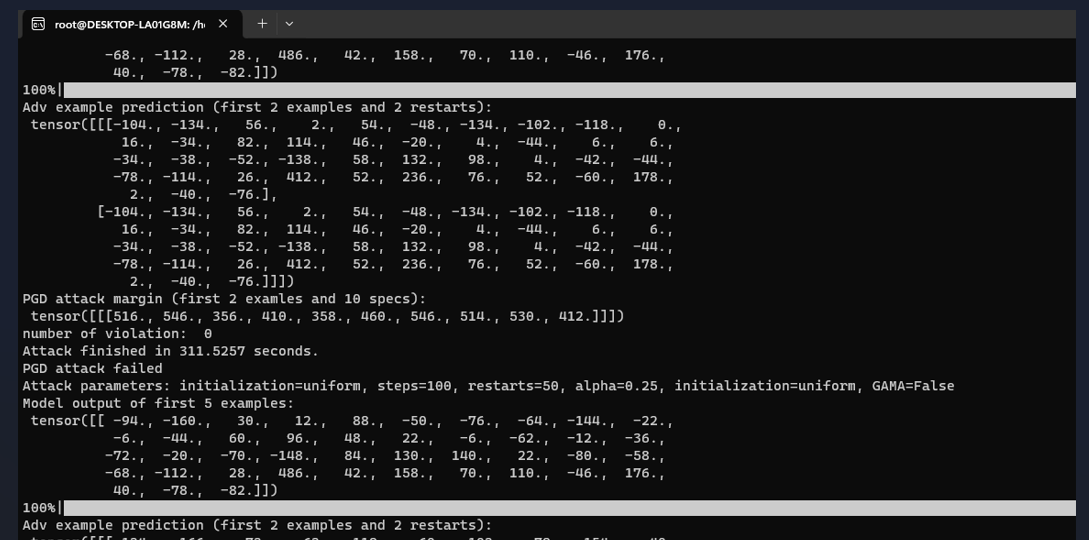
\includegraphics[width=8cm]{7.png}
\end{center}
\end{frame}

\begin{frame}

\frametitle{Rulare benchmark - Alpha Beta Crown}
\tab Rularea se poate face in 2 moduri si anume: cu CPU sau GPU, pentru GPU se foloseste comanda mentionata anterior iar pentru rularea prin CPU de adauga argumentul ”–device cpu”.\\
\tab Executia benchmark-ului poate dura destul de mult timp dar factorul principal care determina timpul este GPU, cu cat este mai performat cu atat va dupa mai putin executia.\\
\tab La finalul executiei se va creea un fisier "out.txt" care contine rezultatul executiei in format binar dupa cum se poate vedea in figura urmatoare:\\
\begin{center}
    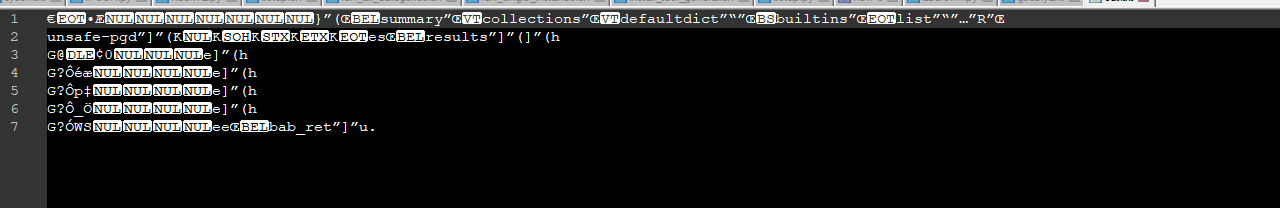
\includegraphics[width=10cm]{6.png}
\end{center}

\end{frame}

\begin{frame}

\frametitle{Rulare benchmark - Marabou}
\subsection{Marabou}
to be done
\end{frame}

\begin{frame}

\frametitle{Bibliografie}
\section{Bibliografie}
\begin{thebibliography}{10}
\addcontentsline{toc}{section}{Bibliografie}
\bibitem{1}
GitHub - Alpha Beta Crown- (\href{https://github.com/Verified-Intelligence/alpha-beta-CROWN}{link})\label{1}

\bibitem{2}
GitHub - Auto LiRPA -  (\href{https://github.com/Verified-Intelligence/auto_LiRPA}{link}) \label{2}

\bibitem{3}
GitHub - Vnncomp2023 (\href{https://github.com/ChristopherBrix/vnncomp2023\_benchmarks}{link})\label{3}

\bibitem{4}
IEEEXplore \label{4}

\end{thebibliography}
\end{frame}

\end{document}